\documentclass[11pt]{article}
\usepackage[margin=1in]{geometry}
\usepackage{amsfonts, amsmath, amssymb}
\usepackage[none]{hyphenat}
\usepackage{fancyhdr}
\usepackage{graphicx}
\graphicspath{ {./media/} }
\usepackage{float}
\usepackage{setspace}
\usepackage{subfig}
\usepackage[nottoc, notlot, notlof]{tocbibind}
%\usepackage{unicode-math}
\usepackage{tabularx}
\usepackage{amsmath} % for boxing equations
\usepackage[font=footnotesize]{caption}
\usepackage{listings}




\pagestyle{fancy}
\fancyhead{}
\fancyfoot{}
\fancyhead[L]{\slshape CALCULATING AREA WITH MONTE CARLO SIMULATIONS}
\fancyhead[R]{\slshape Ben Datsko}
\fancyfoot[C]{\thepage}

\parindent 0ex
%\setlength{\parindent{4em}}
%\renewcommand{\headrulewidth}{0pt}
\renewcommand{\baselinestretch}{1.5}


\begin{document}

\begin{titlepage}
\begin{center}
\vspace*{1cm}
\Large{{IB Mathematics Analysis and Approaches HL}}\\
\Large{Internal Assessment}
\vfill
\line(1,0){400}\\[1mm]
\Large{\textbf{The Monte Carlo Method: An Unconventional Means\\of Calculating Area}}\\
%\Large{\textbf{This is a Sample Subtitle}}\\[1mm]
\line(1,0){400}\\
\vfill
\normalsize Ben Datsko\\
Spring 2021
\end{center}
\end{titlepage}

\tableofcontents
\thispagestyle{empty}
\clearpage

\setcounter{page}{1}

\section{Introduction}
\subsection{Background}
I have decided to focus my exploration on the Monte Carlo method. I was first introduced to this topic while modeling and observing how light interacts with elements in the 3D computer graphics software, Blender. In the real world, when a light source emits a light path, which then collides with another object, the path is scattered/reflected in infinitely many directions (see Figure 1). I assumed Blender took a similar approach to rendering scenes, although I became stumped, as no computer is able simulate infinitely many light paths emanating from a light source. This led me to investigate how computer software like Blender calculates light. I was fascinated to find that computers randomly select a definite number of paths to simulate during the image-rendering process. Because one randomly simulated light path is not valuable on its own, many sample paths can be used to get an accurate idea of the illumination of scenes. Some areas that are hit by many of the randomly generated light rays are brightly-illuminated, whereas other areas that are hit by fewer light rays appear darker. As I investigated, I found the more samples that are generated, the more accurate the image. Thereafter, I learned the mathematical term for this practice: the Monte Carlo method.\\

\begin{figure}[h]
\includegraphics[scale=.15]{marble_box}
\centering\\
\footnotesize\centering Figure 1: An image produced in Blender (annotations made in Photoshop) to denote the behavior of light paths (i.e. raytracing). Rendering parameters: light emits 2000 random sample paths set to collide with 12 surfaces. 
\end{figure}

\normalsize The Monte Carlo method is intriguing as it applies probability and random sampling to numeric problems to form definite solutions. This, juxtaposes the deterministic, formulaic methods I have hitherto used to solve math problems. This then led me to consider irregular shapes, all of which have areas that can be solved through tedious, deterministic, mathematical methods if plotted on a plane with a definite domain. As such, I reckoned it would be interesting to investigate whether it is possible to streamline methods for calculating area through the Monte Carlo method, just as the Monte Carlo method streamlines methods for calculating light in computer programs. Additionally, because I am a technology enthusiast with an interest in software engineering, I sought out to write a program to perform the simulations and generate visual representations of them. Therefore, the aim of this paper is to investigate whether the Monte Carlo method can serve as a viable alternative to deterministic methods of solving mathematical problems.


\subsection{The Monte Carlo Method}

Outside of simulations, obtaining random samples is rife, especially in the sciences. Thus, I will introduce the Monte Carlo method through one such example. Let's say one wants to determine the average height of all people worldwide. In principle, one would need to know the height of every living person to produce an unbiased sample; however, it is impossible to measure the heights of billions of people. Alternatively, one can measure the height of a smaller group of people and hope their average height is a representative of the average height of all people worldwide. However, it is important to note this method only work if performed in a particular way:

\begin{itemize}
  \item Firstly, the selection of the group needs to be unbiased. One can't measure the height of the next 10 people they meet or the height of all their family members, as they may live in an area with especially tall or short people, and because their family may not be representative of the world population. An appropriate method of selecting individuals to form an unbiased sample group is to randomly select people worldwide.

  \item Secondly, the group of measured people must not be too small. If the heights of 5 people are measured, there is a chance that one could have coincidentally picked 5 taller or shorter people. Thus, one can be more confident about the resulting average the more people that are measured. In probability theory, this is referred to as the "Law of Large Numbers."
\end{itemize}

This is, by definition, a working example of the Monte Carlo method, as the goal of a Monte Carlo simulation is to provide a representative group of samples of some large population of possibilities by allowing the simulation to evolve randomly. 

\section{The Area of a Circle}
\subsection{Deterministic Calculations}

First, a sample calculation using the Monte Carlo method will be performed to calculate the area of a circle and demonstrate the properties of the method.
\begin{figure}[h]
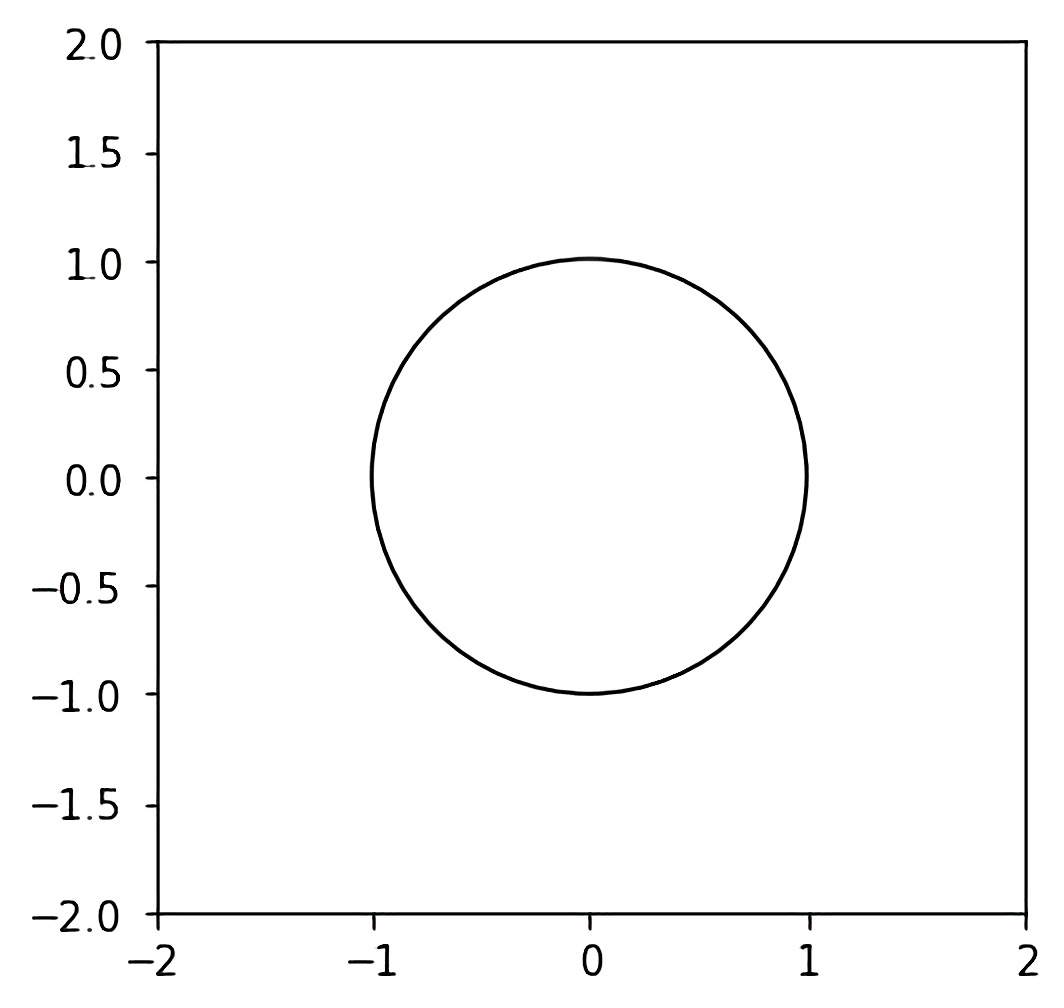
\includegraphics[scale=.2]{circle_clear}
\centering\\
\footnotesize\centering Figure 2: A circle with origin (0, 0) and radius 1; used in sample calculation. 
\end{figure}

Figure 2 provides the radius (1), origin (0, 0) of a unit circle. The equation this circle is, therefore, given by\\[-7ex]

\[(x-0)^2+(y-0)^2=1\]

The domain of possible inputs consists of the square bounded by the x and y axes, as well as the lines x=-2, x=2, y=-2, and y=2, as represented by the square outline in Figure 2. Traditionally, one could use the standard area of a circle equation to find the exact value for the area of the unit circle:\\[-7ex]

\[A=\pi r^2=\pi 1^2 \approx \boxed{\pi}\]
%\[ \boxed{A = 10.265} \]



\subsection{Calculating Using the Monte Carlo Method}
To calculate the area of the circle using the Monte Carlo method, I created a computer program in Python. I chose to create the simulation in Python because it offered me more opportunities to strengthen my programming skills, and because it handles complex mathematical calculations  and graphing far better than other popular programs, like MatLab. Within my program, I included libraries MatPlotLib (which generates graphs) and NumPy (which implements data structures that  are used to store the coordinates of shape vertices). NumPy also offers a 
\texttt{random}
(a function that generates pseudo-random numbers), which produces values that are almost truly random, though, predictability still remains in the random number generation process as a pre-programmed computer algorithm generates them to begin with. I will not go much more in-depth into randomness or what is defined as "true randomness" as it is out of the scope of this paper. The program itself can be found in Appendix A.\\[-2ex]

Understanding the inner workings of the program is crucial for one's understanding of the remainder of the paper. To begin, a finite number of sample points, whose coordinates are randomly generated using the \texttt{random} library, are plotted across the domain. These randomly plotted points comprise the large group of randomly-evolving sample points, as mentioned in section 2.1. Each point's x and y coordinates are then stored in an array (a list, essentially). After all points have been generated, the program iterates through every point in the array, attains its coordinates, and tests whether the point lies inside of the shape. For every point that is inside the shape, 1 is added to a counter labeled \texttt{inside\_shape}. The predicted area of the shape is then calculated by taking the percentage of all the points within the circle that lie across the domain ($ \frac{inside\_shape}{total\_sample\_points}$) and multiplying it by the area of the domain (which, in this instance, is a square with legs measuring 4 units; thus its area measures 16 units$^2$). MatPlotLib then generates a visual representation of the simulation (Figure 3).\\[-5ex]

%\[\frac{InsideShape}{TotalPointsAcrossDomain}*16\]


\begin{figure}[h]
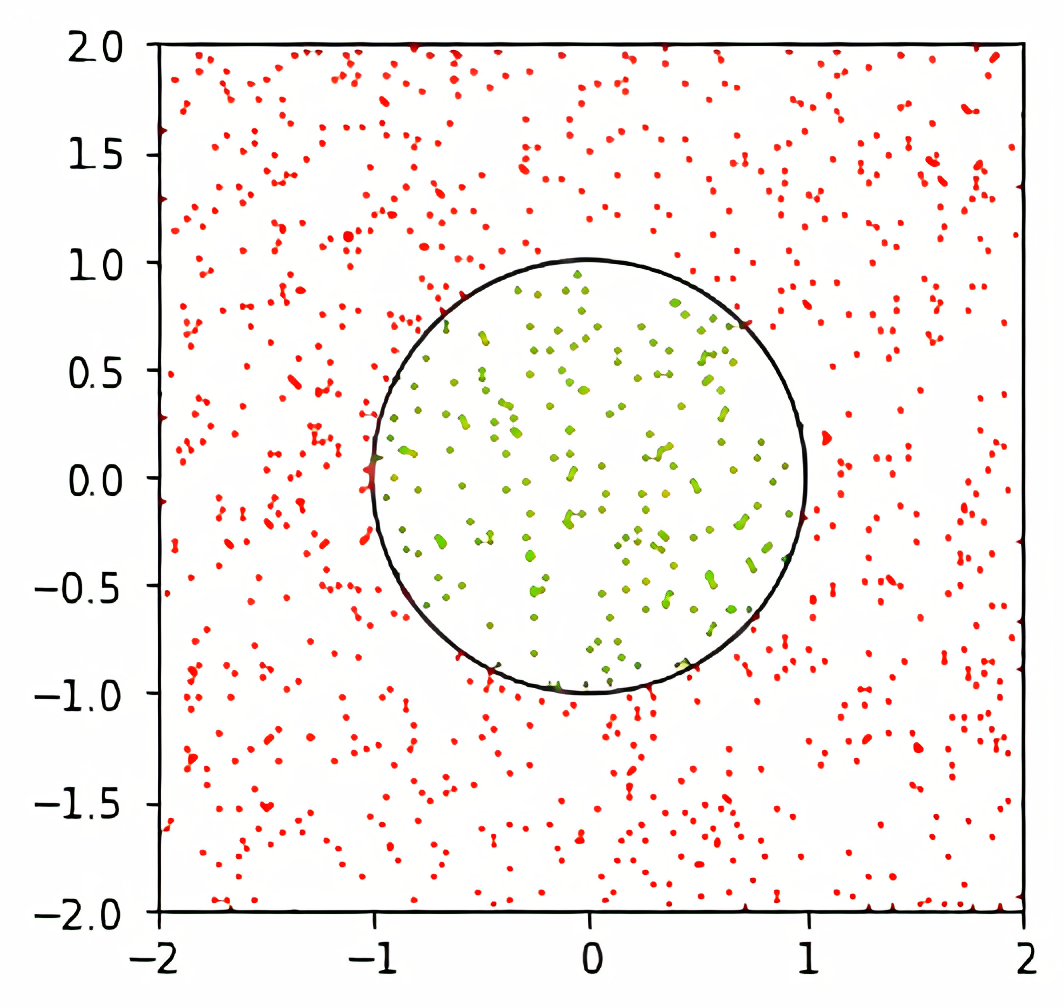
\includegraphics[scale=.19]{circle_populated}
\centering\\
\footnotesize\centering Figure 3: A Monte Carlo simulation plot with 1000 points; generated by the referenced Python program. 
\end{figure} 

\raggedright

\newpage
The table below lists 10 trials, each of which has a different number of generated points and predicted area for the shape. The percent error of each trial is calculated through the standard equation for percent error:\\[-3ex]

\[\frac{|Theoretical-Experimental|}{|Theoretical|}*100\]

 


\begin{table}[H]
    \centering
    \begin{tabularx}{\linewidth}{>{\centering\arraybackslash}X>{\centering\arraybackslash}X>{\centering\arraybackslash}X>{\centering\arraybackslash}X>{\centering\arraybackslash}X }
      \hline \textbf{Number of Points} & \textbf{Points in Circle} & \textbf{Percent of Domain} & \textbf{Predicted Area} & \textbf{Percent Error} \\ \hline
              5                            &	2                         & 40.0\%                      & 6.400                  & 103.72\%            \\ \hline
              10                            &	3                        & 30.0\%                      & 4.800                  & 52.789\%            \\ \hline
              20                            &	5                        & 25.0\%                      & 4.000                  & 27.324\%            \\ \hline
              50                           &	12                        & 24.0\%                      & 3.840                  & 22.231\%            \\ \hline
              100                           &	21                       & 20.9\%                      & 3.340                  & 6.3155\%            \\ \hline
              500                          &	103                       & 20.6\%                      & 3.296                  & 4.9149\%            \\ \hline
              1000                          & 201                      & 20.1\%                      & 3.216                  & 2.3684\%            \\ \hline
              10000                          & 2004                      & 20.0\%                      & 3.206                  & 2.0629\%            \\ \hline
              50000                         & 9890                      & 19.8\%                      & 3.165                  & 0.73871\%            \\ \hline
              100000                         & 19640                     & 19.6\%                      & 3.142                  & 0.02567\%            \\ \hline

    \end{tabularx}\\[2ex]
    \centering\footnotesize Table 1: Predicted area and its accuracy for a varying number of test points.
    \label{tab:data}
  \end{table}
  
It took the computer 183 seconds to generate 100,000 points. Thus, this simulation is capped at 100,000 points for the sake of time and because adding any additional points would produce a negligible difference in the accuracy of the result. Additionally, the area of the unit circle is $\pi$, so proceeding much further would be a futile effort (although it would allow one to estimate additional values of $\pi$ in a rather brute-force manner).\\[3ex]

Clearly, the Law of Large Numbers is supported by Table 1, as the greater the amount of points that are generated, the smaller the percent error, and thus the more accurate the prediction for area. After 100,000 points were used, the percent error became less than one third of a percent.  This, thereby, demonstrates that the Monte Carlo method can accurately estimate the area of shapes.\\


\section{The Area of a Polar Rose}
\subsection{Rationale and Background}

In the previous section, it was disadvantageous to use the Monte Carlo method to calculate the area of the circle, as it required more computing time and power than using deterministic numerical calculation. However, in the case of irregularly-shaped polygons and curved shapes, which have hundreds of degrees of freedom (dimensions), “the curse of dimensionality dictates an exponential increase in complexity as the number of dimensions rises when using deterministic numerical integration.”\cite{dynamicprogramming} Rather, utilizing the Monte Carlo method to calculate the area of such shapes could circumvent the exponential increase in computational time associated with solving through numerical integration. \\[3ex]

To demonstrate the advantages of the Monte Carlo method, I will find the area of a polar rose (Figure 4) using both numerical integration and the Monte Carlo method. The polar rose was selected for this investigation because calculating its area is complex enough to where solving through deterministic means is burdensome, but not ridiculously complicated. 


\begin{figure}[h]%
    \centering
    \subfloat[\centering Cartesian Plane]{{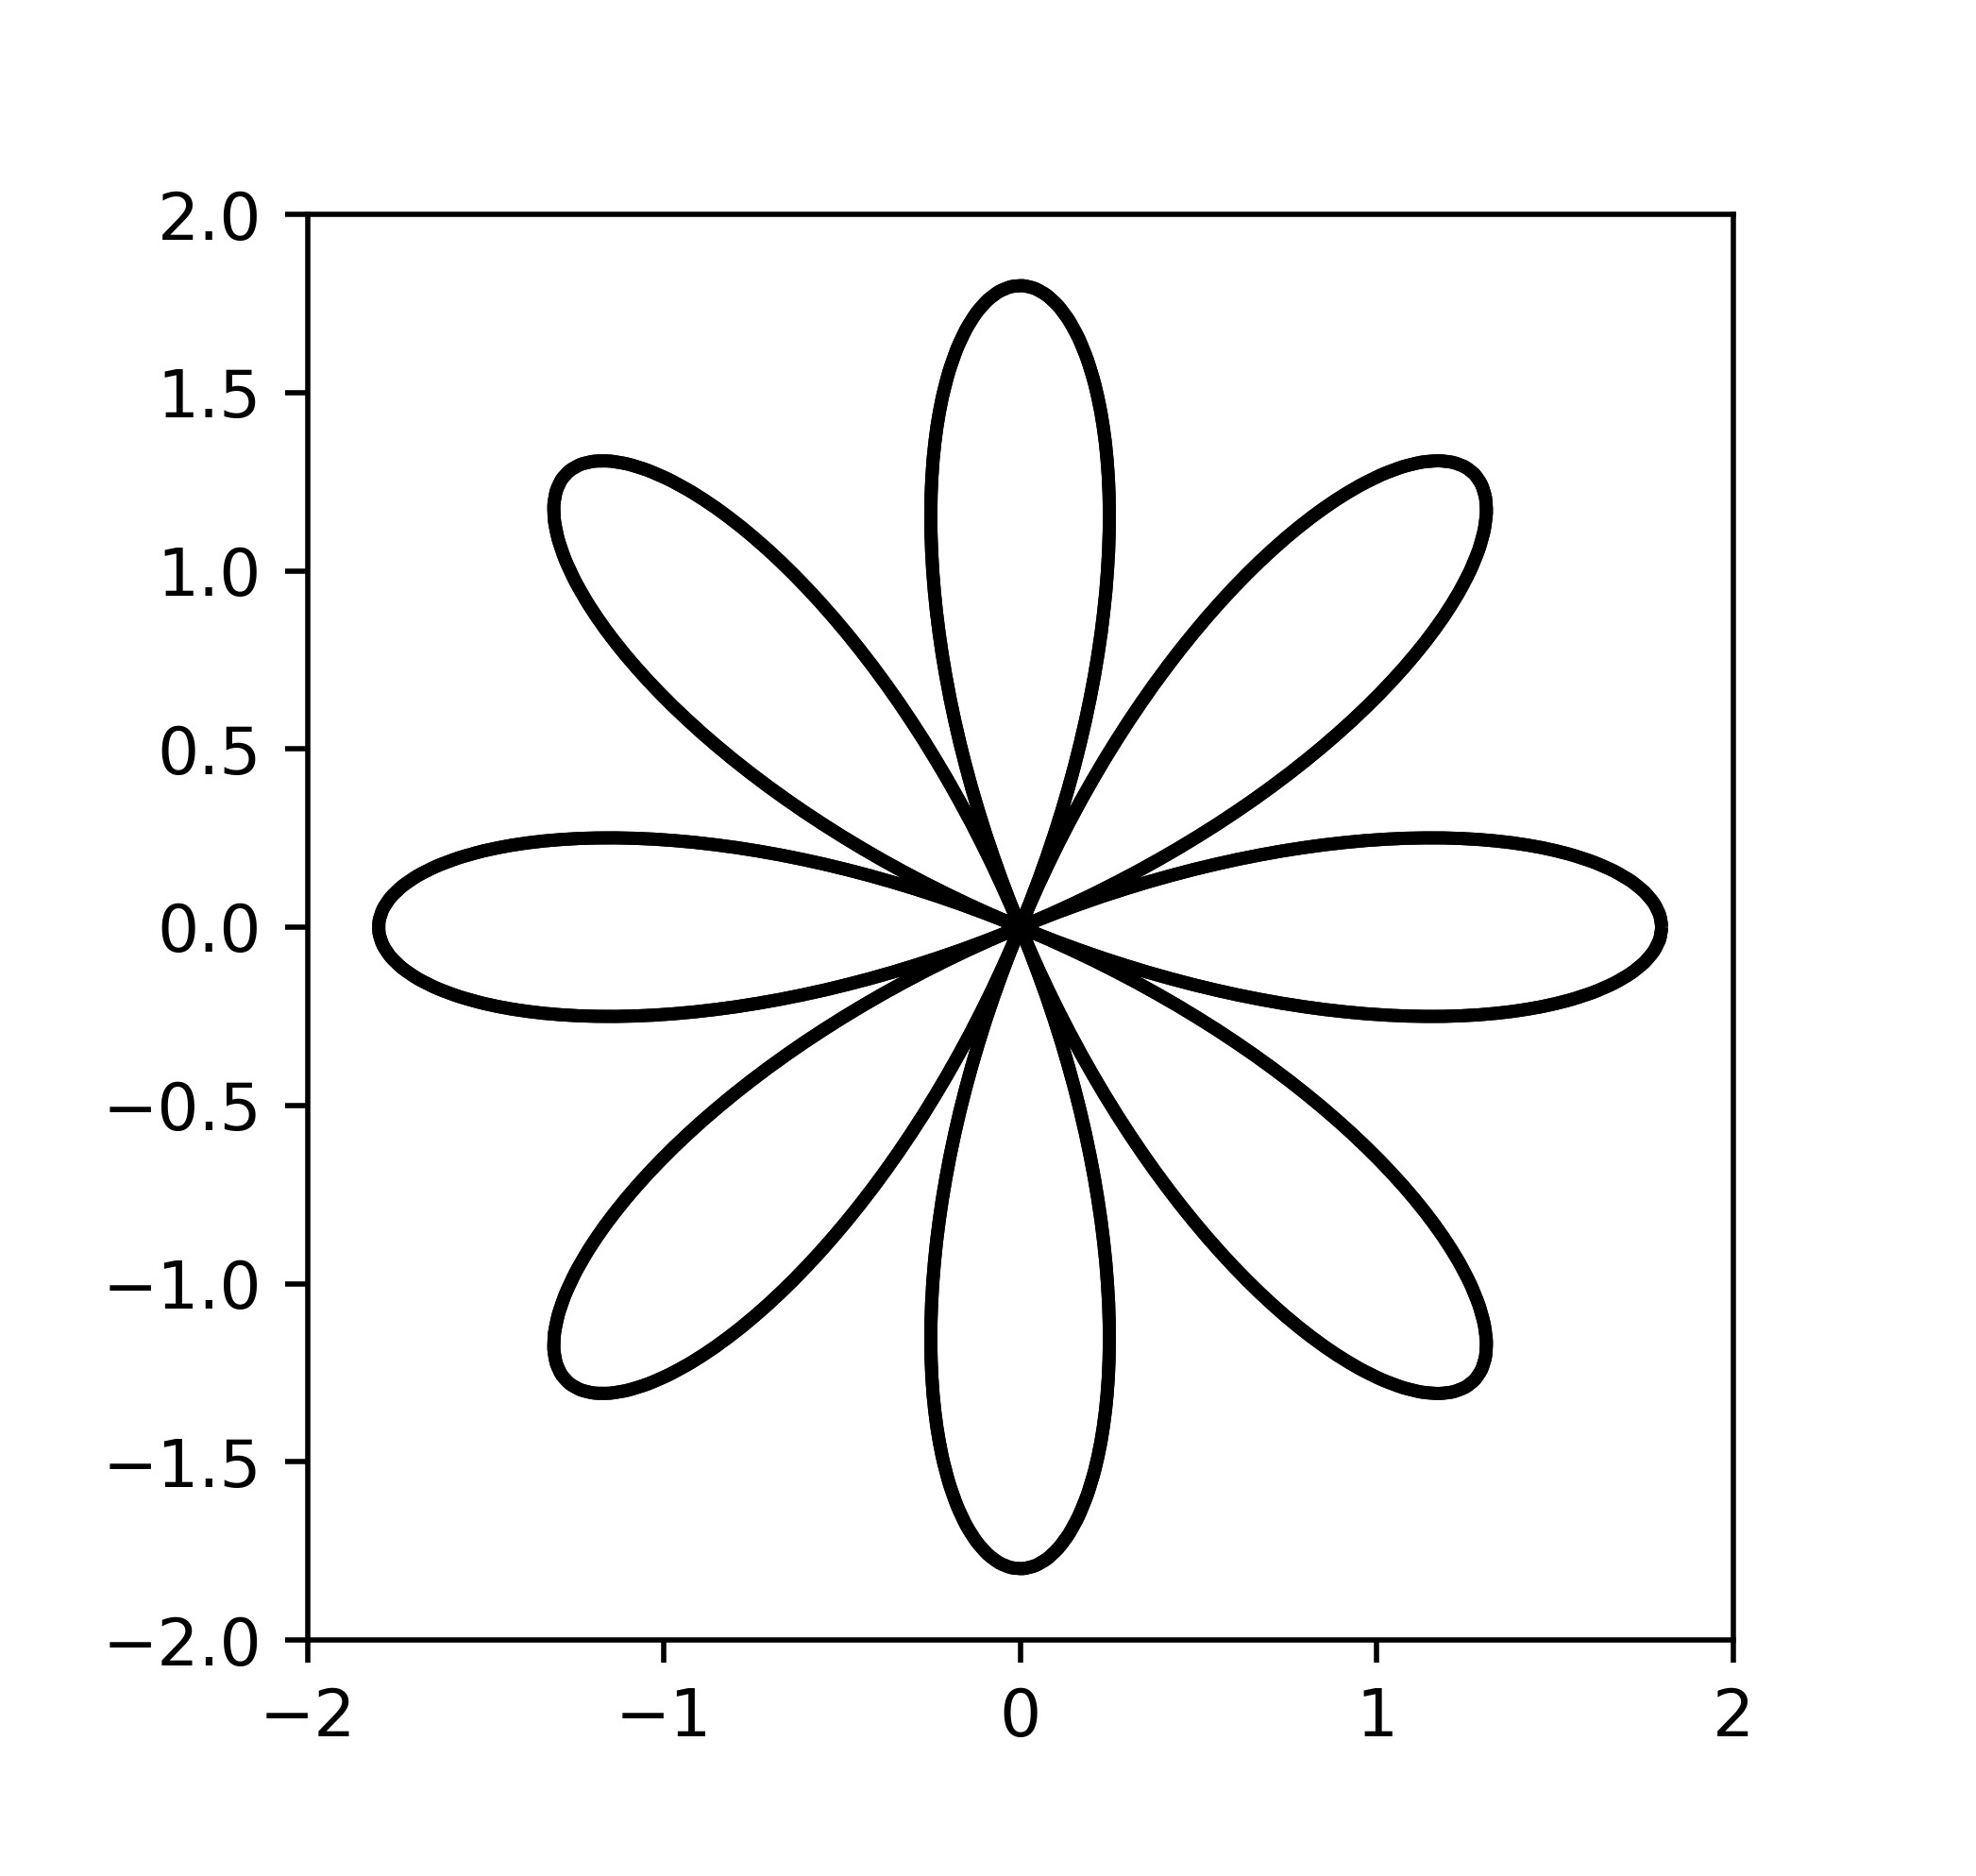
\includegraphics[width=7.5cm]{cartflower} }}%
    \qquad
    \subfloat[\centering Polar Plane]{{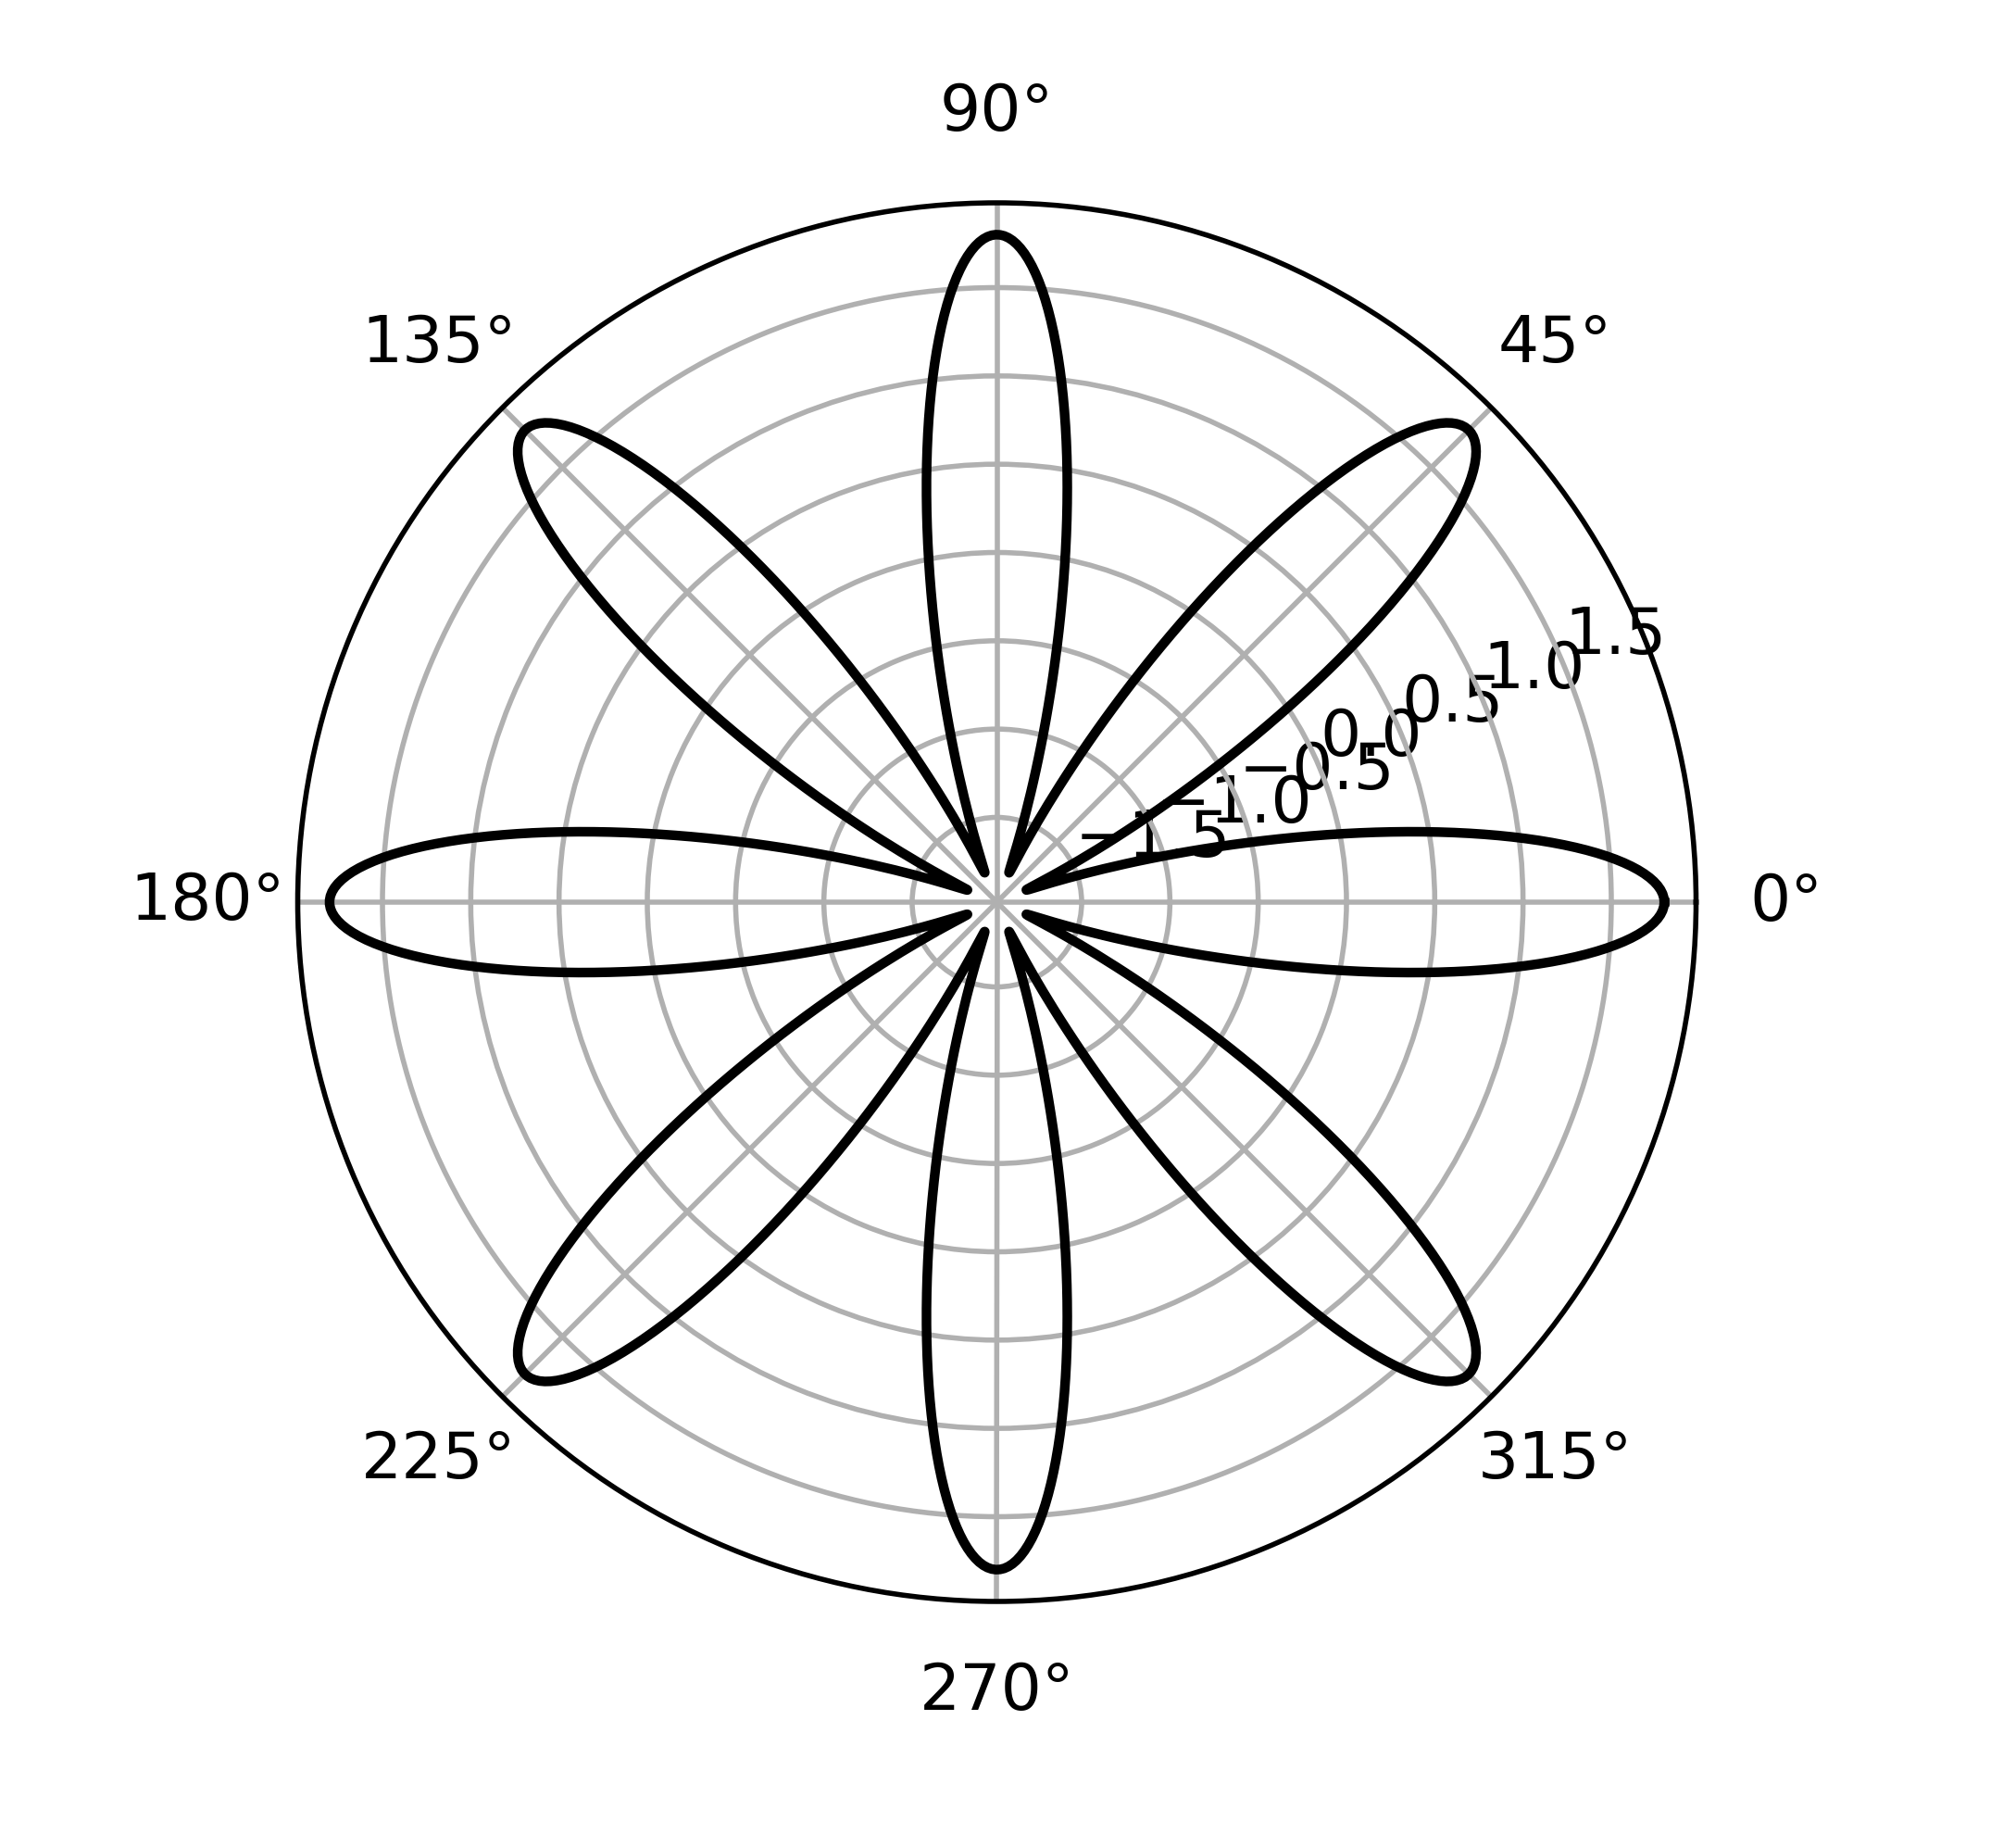
\includegraphics[width=7cm]{polarflower} }}\\[3ex]%
    \footnotesize{Figure 4: A Polar Rose graphed in two different planes.}%
    \label{fig:example}%
\end{figure}

\subsection{Deterministic Calculations}
The equation for the polar rose used in this investigation (Figure 4) is as follows:\\[-3ex]
\[r=1.8*\cos(4\theta)\]
In the equation, 1.8 means that each petal is 1.8 units long, and 4 stands for the number of petals per half of the unit circle. First, it is important to note that the entire shape is composed of duplicates of one petal, all of which are centered at the origin. This means that, to find the area, we simply need to find the area of one petal and multiply it by the total number of petals present. To derive a formula for this, I will consider a circle with radius \emph{r}. As mentioned prior, the standard area of a circle equation is\\[-2ex]
\[A=\pi r^2\]

A sector of this full circle (whose angle measures 2$\pi$) subtending to an angle of $\theta$ would have an area of \\[-2ex]
\[\pi r^2 * \frac{\theta}{2\pi} = \frac{1}{2}r^2\theta\]

This creates a sinusoidal function in the Cartesian plane. Integrating this equation over $\theta_1 \leq \theta \leq \theta_2$ yields the area of swept out of the curve as
\[A_{Petal} \approx \frac{1}{2}\int\limits_{\theta_1}^{\theta_2} r^2 \ d\theta \]
which is the desired formula for the area of one pedal. Given this and the dimensions of the rose, the area can be solved for. Figure 4b informs us that two different pedals in quadrant 1 are bisected by $\theta=0$ and $\theta=\frac{\pi}{4}$. If the areas of these two are combined, they will form the area of one pedal. Knowing this, the bounds for the integral can be set and r can be substituted in to produce the formula representing the area of the function: \\[-2ex]
\[\frac{1}{2}\int\limits_{0}^{\frac{\pi}{4}} (1.8\cos(4\theta))^2 \ d\theta \]
The function can thus be simplified to:
\[\frac{1}{2}(1.8\cos(4\theta))^2 \approx \frac{1}{2}(1.8^2\cos^2(4\theta))\]
\[=\frac{81\cos^2(4\theta)}{50}\]


and can be solved using integration. To begin, I will apply linearity:

\[\frac{81}{50}\int\limits_{0}^{\frac{\pi}{4}} (cos(4\theta)) \ d\theta \]

Now solving: $\int \cos^2(4\theta) \ d\theta$ using u-substitution:

\[Substitute\; u=4\theta \rightarrow \frac{du}{d\theta} = 4 \rightarrow d\theta = \frac{1}{4}du\]
\[=\boxed{\frac{1}{4}\int \cos^2(u)\ du}\]

\newpage
Apply reduction formula for $\int \cos^2(u) \ du$:
\[\int \cos^n(u) \ du=\frac{n-1}{n}\int \cos^{n-2}(u) \ du + \frac{\cos^{n-1}(u)\sin(u)}{n} \rightarrow n = 2\]
\[=\frac{\cos(u)sin(u)}{2} + \frac{1}{2} \int 1 \ du\]

Now solving $\int 1 \ du$

\[\int 1 \ du \rightarrow Apply \ constant \ rule:\]
\[= \boxed{u}\]

Plug in the two solved integrals:
\[\frac{\cos(u)\sin(u)}{2} + \frac{1}{2}\int 1 \ du\]
\[= \frac{\cos(u)\sin(u)}{2} + \frac{u}{2} \]
\[\therefore \ \frac{1}{4}\int \cos^2(u)\ du = \frac{\cos(u)\sin(u)}{8} + \frac{u}{8} \]
Undo u-substitution by replacing \emph{u} with $4\theta$
\[=\frac{cos(4\theta)\sin(\theta)}{8} + \frac{\theta}{2}\]

Plug back into initial integral, $\frac{81}{50}\int\limits_{0}^{\frac{\pi}{4}} (cos(4\theta)) \ d\theta $:
\[=\frac{80cos(4\theta)\sin(\theta)}{400} + \frac{81\theta}{100}\]

Simplify and rewrite for the final answer:
\[\frac{81(\sin(8\theta)+8 \theta) + 80}{800} + C\]

\newpage
When $\frac{\pi}{4}$ is plugged in for theta (C can be ignored because this integral is definite) we get the area of one rose petal. This can then be multiplied by 8 for the total area of the rose:

\[\frac{81 \pi}{400} * 8 = \boxed{5.089 \ units^2}\]

\section{Solving Using the Monte Carlo Method}

The polar rose used in this investigation is in the Cartesian plane (Figure 4a) as opposed to the Polar plane (Figure 4b). This is done for the sake of consistency, as the circle from section 2 is in the Cartesian plane. However, because polar functions are plotted in the Polar plane by default, I began by plotting the rose using the aforementioned formula\\[-3ex]

\[r=1.8*\cos(4\theta)\]

The coordinates produced then connected via Bezier curves generated by Python’s MatPlotLib library to form an image in the polar plane (Figure 4b). I made sure to store the polar x- and y-coordinates of the points of every point used to create the rose in separate lists. I was then able to iterate through all 1000 polar points in each list, and then, because polar points are formatted as (r, theta), convert them to their corresponding values on the Cartesian plane using the following equation:\\[-3ex]

\[X_{Cartesian}=r*\cos(\theta)\]\\[-7ex]
\[Y_{Cartesian}=r*\sin(\theta)\]


I then graphed every translated polar point onto the Cartesian plane to produce the Cartesian version (Figure 4a). 

\begin{figure}[h]
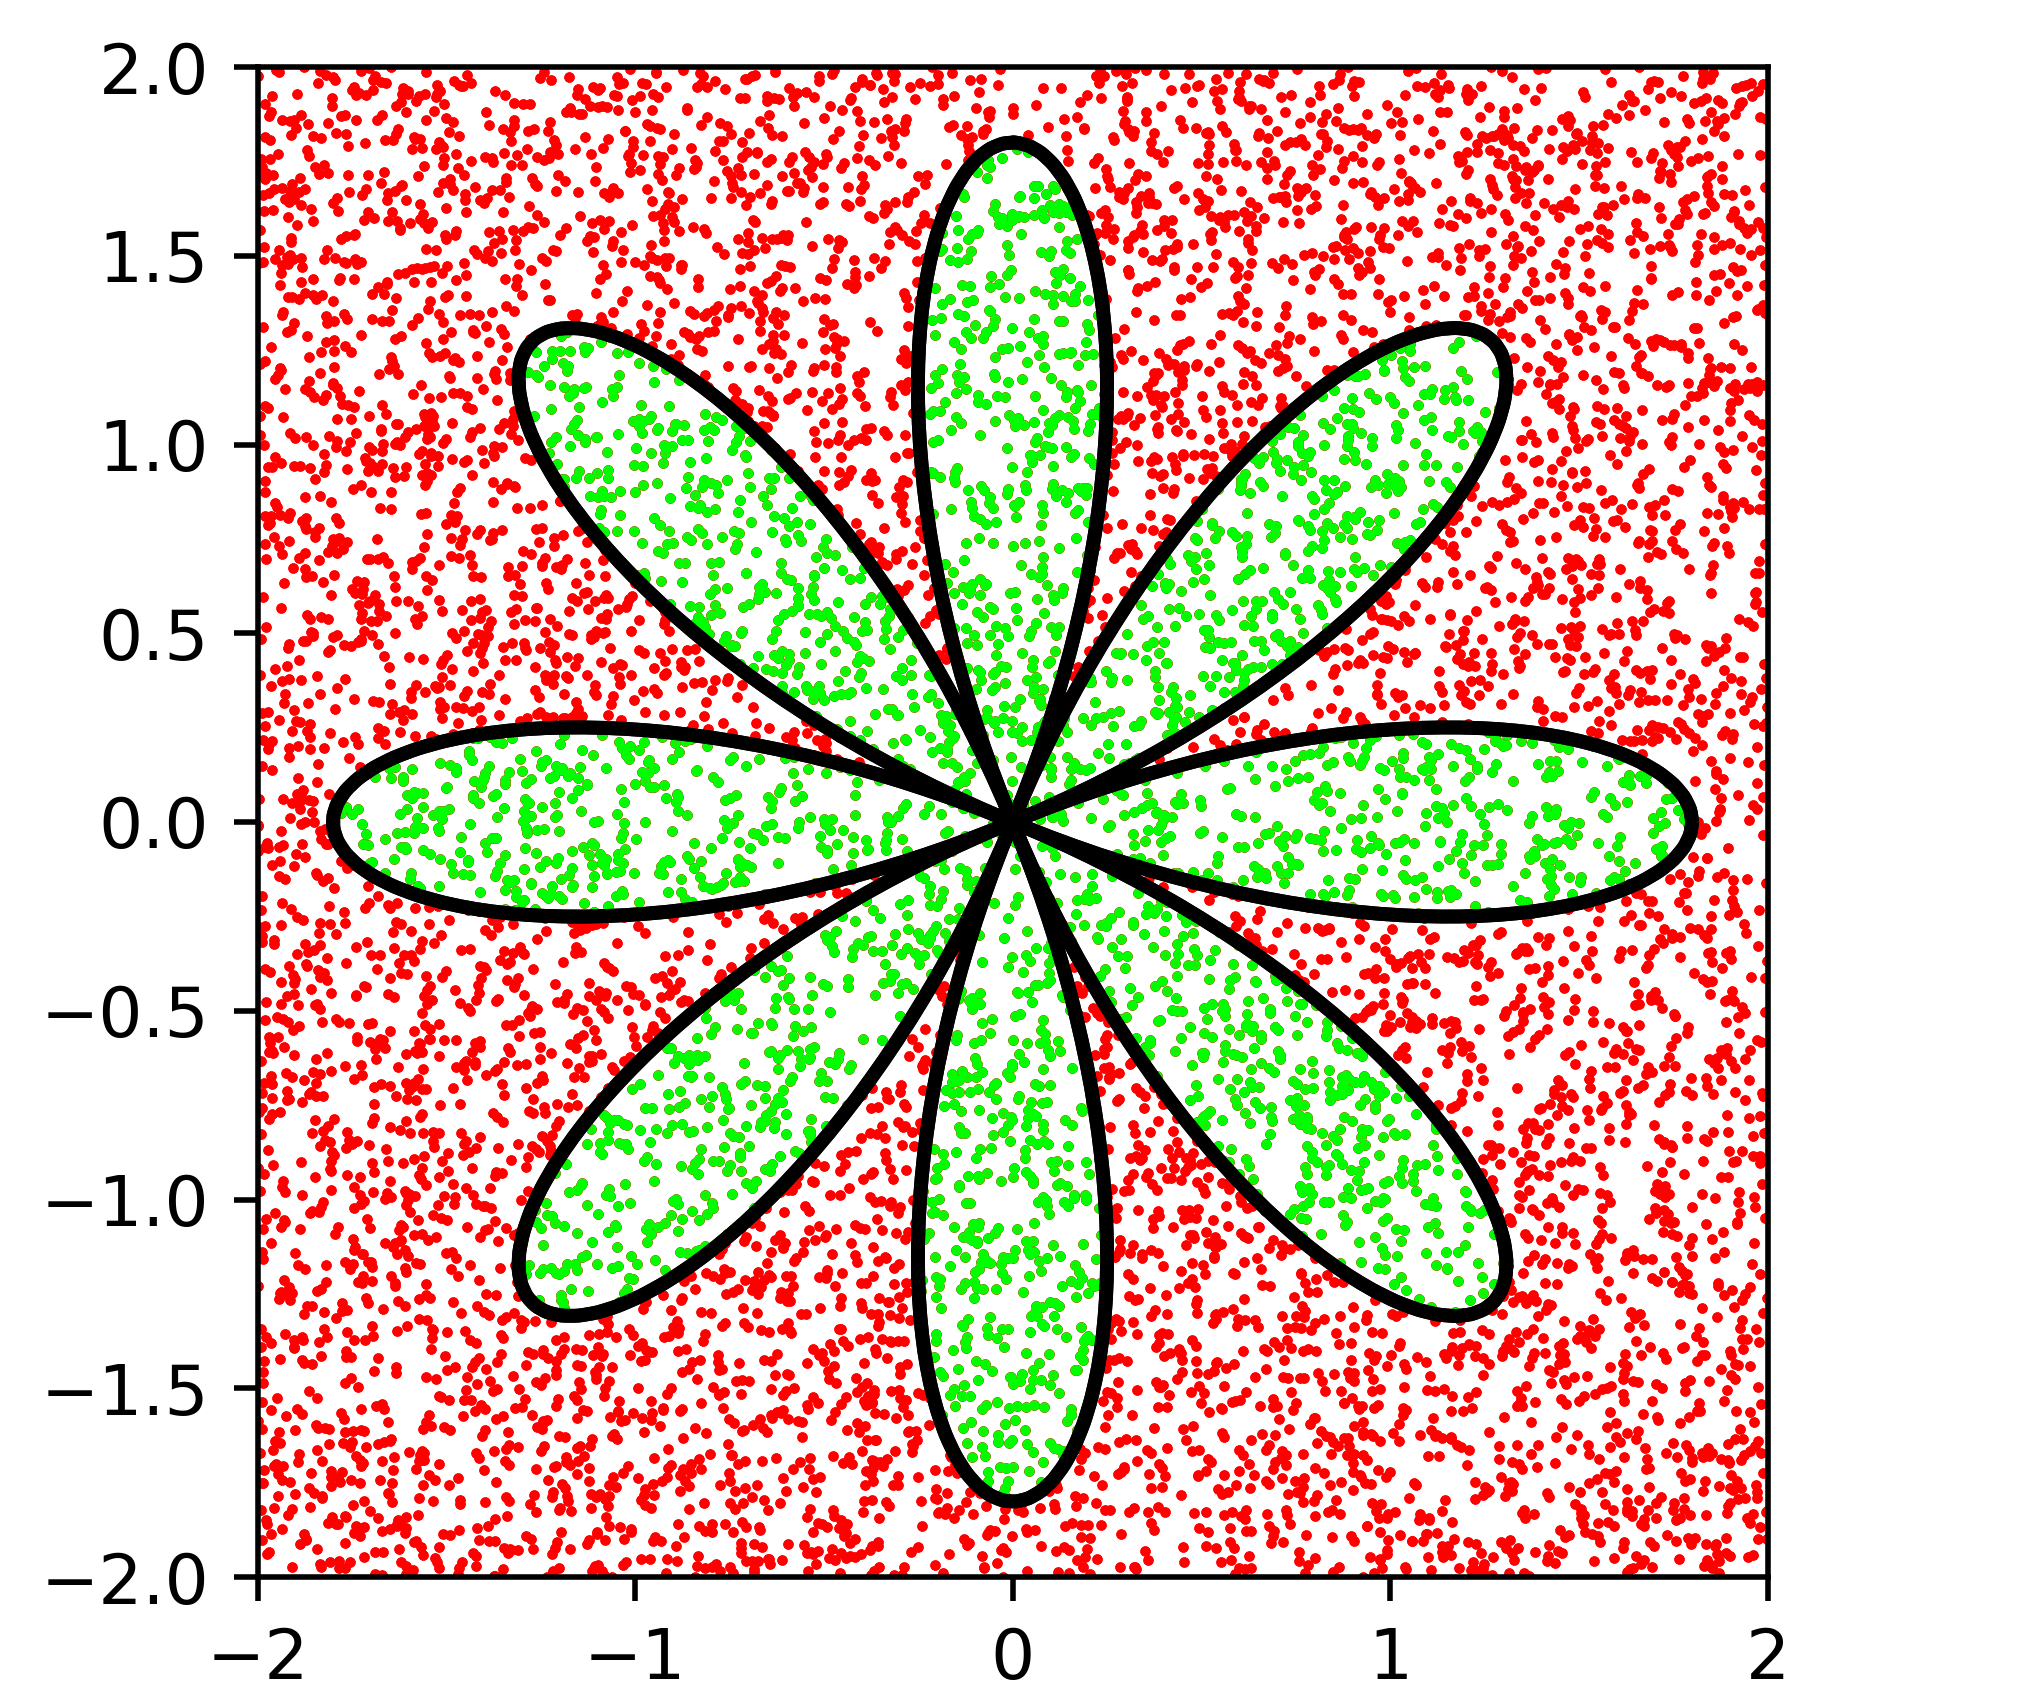
\includegraphics[scale=.2]{monte_carlo_rose}
\centering\\
\footnotesize\centering Figure 5: A render produced by the program of the simulation at 10,000 points.
\end{figure}

It took a computer 332 seconds to generate 100,000 points. As shown in Table 2, the percent error diminishes as more and more points are generated. At 100,000 data points, the percent error is negligible.

\begin{table}[H]
    \centering
    \begin{tabularx}{\linewidth}{>{\centering\arraybackslash}X>{\centering\arraybackslash}X>{\centering\arraybackslash}X>{\centering\arraybackslash}X>{\centering\arraybackslash}X }
      \hline \textbf{Number of Points} & \textbf{Points in Circle} & \textbf{Percent of Domain} & \textbf{Predicted Area} & \textbf{Percent Error} \\ \hline
              5                            &	3                         & 60.0\%                      & 9.6                  & 88.63\%            \\ \hline
              10                            &	5                        & 50.0\%                      & 8                  & 57.19\%            \\ \hline
              20                            &	8                        & 40.0\%                      & 6.4                  & 25.75\%            \\ \hline
              50                           &	13                        & 26.0\%                      & 4.16                  & 18.26\%            \\ \hline
              100                           &	30                       & 30.0\%                      & 4.8                  & 5.69\%            \\ \hline
              500                          &	163                       & 32.6\%                      & 5.216                  & 2.49\%            \\ \hline
              1000                          & 333                      & 32\%                      & 5.12                  & 0.6016\%            \\ \hline
              10000                          & 3168                      & 31.68\%                      & 5.0688                  & 0.4044\%            \\ \hline
              50000                         & 15932                      & 31.864\%                      & 5.09824                  & 0.1741\%            \\ \hline
              100000                         & 31807                     & 31.807\%                      & 5.08912                  & 0.00510\%            \\ \hline

    \end{tabularx}\\[2ex]
    \centering\footnotesize Table 2: Predicted area and its accuracy for a varying number of test points.
    \label{tab:data}
  \end{table}

Therefore, it can be said that, in this example, where the area of the polar rose is calculated, it is much simpler and less time-consuming to use the Monte Carlo method rather than using integration to solve the area of the shape. Setting up the expression, determining the limits of integration, and solving requires a hefty amount of calculation, whereas generating 100,000 points with a computer program and utilizing the Monte Carlo method produced the same answer of $5.089 \ units^2$ in far less time. Thus, for complex shapes, using the Monte Carlo method to solve for area is advantageous over conventional methods of solving.

\section{Applications}

Clearly, using the Monte Carlo method to solve for area is advantageous. This also means the Monte Carlo method can provide a viable alternative to calculating the volume of complex 3D figures deterministically, the process of which is even more complicated than calculating the area of complex shapes. The Monte Carlo method has many applications in the real world as well. In engineering fields like industrial design, software, such as Catia V6, uses the Monte Carlo method for calculating the volume of complex shapes, for ray tracing during model rendering, and for part tolerance testing. Tolerance is the total amount a dimension in a part (a model that composes an assembly of parts; a vehicle, for instance, is an assembly) may vary, and is the difference between the upper (maximum) and lower (minimum) limits. Catia V6 uses the Monte Carlo method to  generate a vast number of assemblies, each of which has parts with slightly different dimensions. These parts are then assembled, and a compatibility rating is outputted for each model. This allows engineers to calculate part tolerance,  which is then used to control the amount of variation present in all manufactured parts.\cite{catia}\\[3ex]

Additionally, Monte Carlo simulations are used in economics to predict the future performance of markets given historical data. One such example of a market performance predictor that uses a Monte Carlo simulation is the application cFIRESim. This product considers Consumer Price Index inflation (the average change in price over time consumers pay for a good), the value of the user's portfolio, their retirement time frame, yearly spending, and yearly income \cite{cfiresim} to predict the geometric mean of the growth of the user's portfolio, and aid them in their decision-making process.  

\section{Conclusion}
I began this investigation with the intention to investigate what allows computer modeling software to be performant, as well as the Monte Carlo method (as I had never heard of it); however, I came out with much more. First, through taking a deep dive into the Monte Carlo method, as well as its plethora of practical applications and the multitude of ways in which revolutionized the fields of science, economics, and engineering, I could learn more about the world. Second, this investigation provided me with an opportunity to link up my math coursework with my hobbies—graphic design and computer science—and learn new skills. \\[3ex]

Altogether, I believe that through investigating Monte Carlo simulations, I have grown as a mathematician. I have been taught that contrary to popular belief, creativity is involved in mathematics. In other words, I learned there is never one way to solve a mathematical problem, and that the conventional approach to solving a problem doesn't necessarily mean that it is the best approach. Thus, I have broadened my ability to solve deterministic problems in an unconventional manner (i.e. I have improved my critical thinking skills). With my new knowledge, I can better appreciate the widespread application of mathematics in my daily life. I believe the multidisciplinary nature of this investigation will lead me to continue to research this topic, as I have experience in and will continue to work in many fields that are impacted by this method. 


\newpage

\begin{thebibliography}{9}
\bibitem{dynamicprogramming} 
Bellman, R. E. (2010). \emph{Dynamic Programming}. Princeton, NJ: Princeton University Press.

\bibitem{catia}
Catia V6 Integrated Tolerance and SPC Systems. (n.d.). Retrieved March 03, 2021, from https://www.3dcs.com/en-gb/tolerance-analysis-software-and-spc-systems/catia-v5-integrated\#:~:text=\\The\%20Leading\%20Variation\%20Analysis\%20Solution,\%2DMean\%20(Sensitivity)\%20Analysis.

\bibitem{cfiresim}
CFIRESim. (n.d.). Retrieved March 03, 2021, from https://www.cfiresim.com/


\end{thebibliography}

\newpage

\appendix


\section{Appendix: Python Code for the Monte Carlo Program}



\begin{singlespace}
\begin{lstlisting}
import numpy as np
import matplotlib.pyplot as plt
from matplotlib.patches import Circle
from matplotlib.path import Path
import matplotlib.patches as patches
import time

# Define timer

then = time.time()

# ==============================================
#                   SHAPES
# ==============================================

# ####################################
# #    Circle (uncomment to use)
# ####################################
# Create the initial circle
circle = Circle([-1,-1], radius=1)

# Get the path
path = circle.get_path()
patch = patches.PathPatch(path, facecolor='none', edgecolor='#000000')

## ####################################
## #   Polar Rose (uncomment to use)
## ####################################

# Plot in polar coordinates

theta = np.linspace(0, 2 * np.pi, 1000)  # generate 1000 points in a circle (hence 2pi)

r = 1.8 * np.cos(4 * theta)  # funtion

# convert to cartesian

xcart = r * np.cos(theta)
ycart = r * np.sin(theta)

newarrx = np.array_split(xcart, 1000)
newarry = np.array_split(ycart, 1000)

verts = [None] * 1000
codes = [None] * 1000

i = 0
while i < 1000:
    verts[i] = (float(newarrx[i]), float(newarry[i]))
    codes[i] = Path.CURVE4
    i = i + 1

codes[0] = Path.MOVETO

path = Path(verts, codes)

(fig, ax) = plt.subplots()
patch = patches.PathPatch(path, facecolor='none', lw=2)
ax.add_patch(patch)

##################
#  Scatter Plot
##################

# Total number of random points

total_random_points = 5

# Create empty x and y arrays for eventual scatter plot of generated random points

x_plot_array = np.empty(shape=(1, total_random_points))
y_plot_array = np.empty(shape=(1, total_random_points))

# Create random values (x,y) between -1 and 1

x = np.random.uniform(-2, 2, size=total_random_points)
y = np.random.uniform(-2, 2, size=total_random_points)

# Plot output of random points and circle

random_points_plot = plt.scatter(x, y, color='red', s=.25)
random_points_plot.set_zorder(0)  # set scatter plot position to back

# ==============================================
#           MONTE CARLO CALCULATIONS
# ==============================================

inside_shape = 0

# Iterate over points to locate them and count points inside unit circle

for i in range(0, total_random_points):

    # locates the points

    x_2 = x[i]
    y_2 = y[i]

    # Tests for whether the specified point is contained by the shape

    result = str(path.contains_points([[x_2, y_2]]))

    # Count if inside shape

    if '[ True]' == result:
        inside_shape = inside_shape + 1  # Add 1 to the counter
        plt.scatter(x[i], y[i], color='lime', s=.25)  # Change the color of the point to green

# Stats: Number of points inside shape compared to total

in_to_out_ratio = inside_shape / total_random_points

# ==============================================
#                    DRAW
# ==============================================
# Create axis with equal aspect ratio in both axis

ax = plt.gca()
ax.set_aspect('equal', 'box')

# Set axis limits

ax.set_xlim((-2, 2))
ax.set_ylim((-2, 2))

# Add the points and the shape to the plot

ax.add_artist(random_points_plot)
ax.add_patch(patch)

# Render plot in screen

plt.show()

# End timer

now = time.time()

# Log stats in console

print '\n--------------'
print '\n Statistics'
print ('\n Total number of points on graph:', total_random_points)
print ('\n Area of graph:', 16)
print ('\n IN OUT RATIO:', in_to_out_ratio)
print ('\n Number of points inside shape:', inside_shape)
print ('\n Area of shape:', in_to_out_ratio * 16)  # Multiplying probability by total area to find area of sector
print ('Calculation performed in: ', now - then, ' seconds')

\end{lstlisting}
\end{singlespace}



\end{document}
